\subsection{Output}
We designed the software to output individual car journeys for a transport consultant to analyse using statistical analysis packages.  The basic idea is that the software is used to support decisions about  changes to the road network or for supporting planning decisions.  We present two scenarios here. Instead of using a statistical analysis package such as SPSS we wrote a custom python script to summarise the data.  The script also serves as a sanity check for the output of our software.  The python script is included in the appendix to this report. 



\subsubsection{Shopping Centre Development}
We have a simple network as shown below.  The consultant does a survey to measure existing traffic movements which we translate into a \textit{demand matrix} for the road system.  The demand matrix is just a count of car movements between each end point of the network over a given time period.  We are keeping things simple in our example and only considering one vehicle type.  In reality the model would take into account of other vehicle types and our software does allow for that.  We convert this demand matrix into a table which specifies the probability of a car entering the network at for each combination of origin and destination for each tick of the simulation clock.  This drives the creation of vehicles in our simulation for the base case.  \\ The consultant runs other models, based on the size of the new shopping centre and proximity of other centres to estimate a new demand matrix for when the centre is built.  Our software is then run in the base case and the modelled case using the new demand matrix and reports are generated showing the effect on journey times.\\ \textbf{Network diagram}
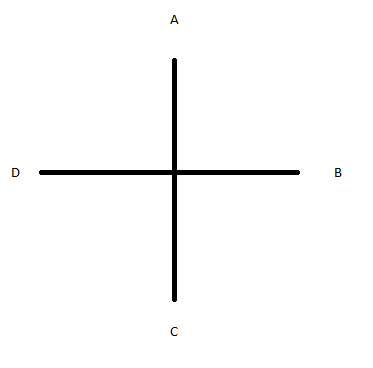
\includegraphics[scale=0.5]{./images/network.png}

We used the following trip matrix for the base case:
	\begin{center}
	\begin{tabular}{| c | c | c | c | c |}
		\hline
		\textbf{ }	&	A & B & C & D \\ \hline
		A				&	0 & 0.3 & 0.3 & 0.3				\\ \hline
		B					&	0.3 & 0 & 0.3 & 0.3				\\ \hline
		C	&	0.3 & 0.3 & 0 & 0.3			\\ \hline
		D				&	0.3 & 0.3 & 0.3 & 0				\\ \hline

		
	\end{tabular}
	\end{center} and the following matrix, showing extra demand to and from the shopping centre at C
    \begin{center}
	\begin{tabular}{| c | c | c | c | c |}
		\hline
		\textbf{ }	&	A & B & C & D \\ \hline
		A				&	0 & 0.3 & 0.8 & 0.3				\\ \hline
		B					&	0.3 & 0 & 0.8 & 0.3				\\ \hline
		C	&	0.5 & 0.5 & 0 & 0.5			\\ \hline
		D				&	0.3 & 0.3 & 0.8 & 0				\\ \hline

		
	\end{tabular}
	\end{center}
    
    The output shows the expected behaviour:  proportionally more cars going to and from C and the average journey times to C increased.  The output for the two cases is shown below\\ \textbf{Base case}\\
    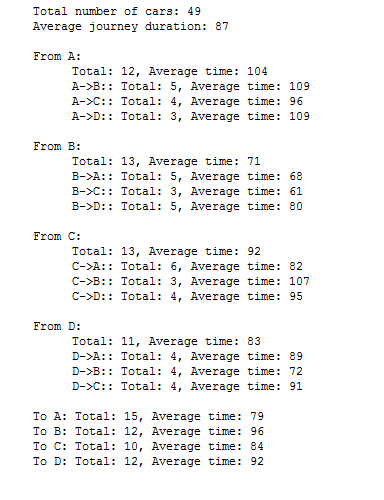
\includegraphics[scale=1.0]{./images/scenario1.png}\\ \textbf{Planned Shopping Centre}\\
    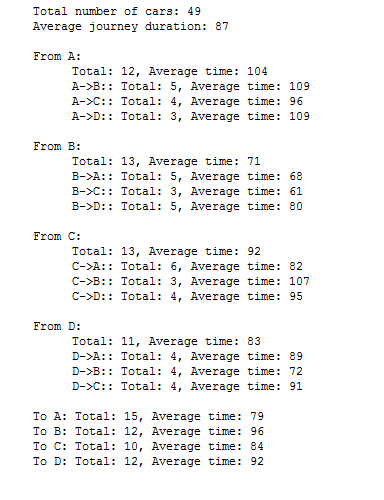
\includegraphics[scale=1.0]{./images/scenario2.png}
    
    
\subsubsection{Congestion Charge}
This scenario is similar to the Shopping Centre example but this time we are reducing demand for journeys to one node in the network by introducing a toll in the road system.  We should see a reduction in journey times as congestion is reduced.
   
    

In this case we used the following trip matrix and got the output below, which supports the case for a congestion charge at C reducing journey times
 \begin{center}
	\begin{tabular}{| c | c | c | c | c |}
		\hline
		\textbf{ }	&	A & B & C & D \\ \hline
		A				&	0 & 0.5 & 0.1 & 0.3				\\ \hline
		B					&	0.3 & 0 & 0.1 & 0.3				\\ \hline
		C	&	0.3 & 0.3 & 0 & 0.3			\\ \hline
		D				&	0.3 & 0.5 & 0.1 & 0				\\ \hline

		
	\end{tabular}
	\end{center}
~ \\ \textbf{Planned Shopping Centre}\\
    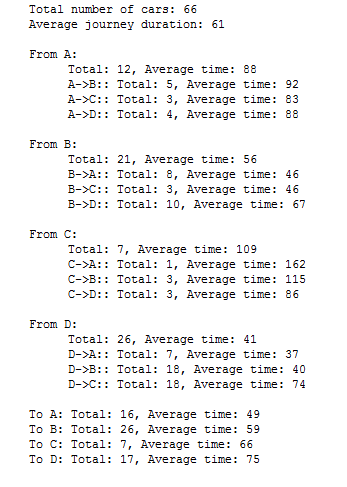
\includegraphics[scale=1.0]{./images/scenario3.png}
